\documentclass[a4paper,%            A4 papir size
               aps,%                Document gets APS layout
               prl,%                more layout, section numbering is removed
               amsfonts,%           load AMS fonts
               amssymb,%            load more AMS symboler
               amsmath,%            load AMS math (equation environment and so on...)
               nobibnotes,%         If BibTex is not used, REVTeX should be told to use normal footnotes
               twocolumn, %         two-column layout
               twoside,%            to-sided print
               balancelastpage,%    balancing the last page when using two columns
               eqsecnum] %          numbering the equations with the sectionnumber
               {revtex4-1}
\usepackage[utf8]{inputenc}
\usepackage[english]{babel} 


\usepackage{amsmath, amssymb}
\usepackage{url}
\usepackage{wrapfig}
\usepackage{subfiles}
\usepackage[squaren]{SIunits}
\usepackage{caption}
\captionsetup{labelfont={footnotesize,bf},textfont=footnotesize,format=hang,indention=-0.5cm} 
\usepackage[normalem]{ulem}
\usepackage{subfigure}
\usepackage{lipsum}
\usepackage{todonotes}
\usepackage{float}
\usepackage{hyperref}

\begin{document}                                
\selectlanguage{english}

\date{December 15, 2021}
\title{Applied Statistics - Project}
\author{Ariel Avanzi}
\author{Alexander Buhl}
\author{Patrizio Cugia di Sant'Orsola}
\author{Svend V. Korsgaard}
\author{Nathánaël van den Berg}

\affiliation{Niels Bohr Institute - Applied statistics - Project group 12}


\begin{abstract}                                              
This paper presents a study on $g$, the gravitational constant acceleration obtained in two different and independent ways. We begin by obtaining it using a pendulum, whose period and length are measured in the laboratory, that results in the value: $g_{pendulum}=(9.82 \pm 0.04)\frac{m}{s^2}$. $g$ is later calculated again using a ball rolling down an incline, and considering the relation between gravity and its acceleration. This method yields results that are inconsistent between measurements.
\end{abstract}

\maketitle 

\section{Introduction}


The aim of this project is to estimate the value of $g$, the gravitational acceleration, using two different set ups,  trying to calculate it with the highest possible accuracy and precision. 
The first experimental set up is a pendulum, after measuring the length of the pendulum $(T)$ and its period $(g)$ is obtained as: $g=L(\frac{2 \pi}{T})^{2}$, using the relation: $T=2 \pi\sqrt{(\frac{L}{g})}$, which is derived from newton's laws of motion.
The second method makes use of a ball rolling down an incline to get the value for $g$. The ball rolls down the inclined track, where the acceleration is estimated thanks to five light sensors placed on the track, that combine the passing timings of the ball and the distance covered to estimate the acceleration $a$. 
$g$ is then obtained as $g=\frac{a}{\sin{(\theta+\Delta\theta)}}[1+\frac{2}{5}\frac{D_{ball}^2}{D_{ball}^2-D_{rail}^2}]$.
The experimental set is represented in figure \ref{fig:pendulumfit}, where $a$ is the acceleration of the ball, $\theta$ is the angle of the incline relative to the table, $\Delta\theta$ is the angle between the table and the flat level, and $D_{rail}$ and $D_{ball}$ are the respective diameter of the rail track and the rolling ball. 

\begin{figure}[h]
\centering
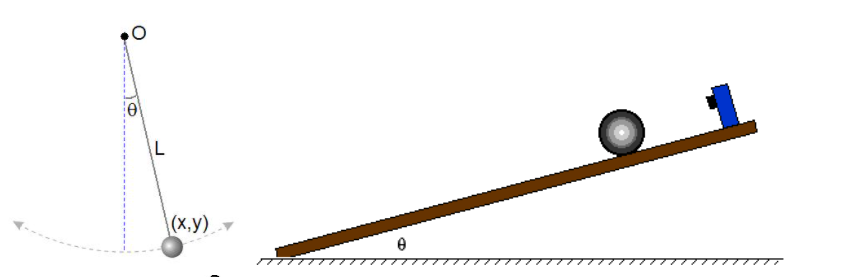
\includegraphics[width=\linewidth]{setup12.PNG}
\caption{The setups for both the pendulum (left), and the ball on incline (right), image courtesy of \cite{setup}. \label{setupfig}}
\end{figure}

\section{Method}
The measurements referred to in the following article have been taken independently by different group members. The errors are also estimated independently, taking into account not only the accuracy of the instrumentation, but also the various factors depending on the environment and the experimental set up. 

\subsection{Pendulum}

The first measurements done in this process are on the length and period of the Pendulum. The length $L$, distance from the hook to the center of mass of the mass, is measured in two different ways, using both a $20 \, m$ measuring tape and a laser measuring device.

The laser device is placed near the hook and pointed at the floor as closely as possible to the mass.
A second measurement is made from the floor to the bottom of the weight.
The distance between the weight and the floor can be subtracted from the distance between the hook and the floor. This can be used to calculate the pendulum length in combination with the center of mass position of the weight.
The mass has a cylindrical shape, and its height was measured with a caliper.
The measuring tape pendulum length was measured from the hook to the top of the weight.
%These measures can be combined to obtain the final value for $L$. 
%To obtain $L$ the measures in table \ref{tab:pendulum} are used.
%The first $L$ is the distance from the hook to the bottom of the mass subtracted half the height of the cylindrical mass, from which: $L_{tape}=(18.47 \pm 0.01)$ m.
%The second $L$ is the distance from the hook to the bottom of the floor, minus half of the height of the mass and the distance from the bottom of the floor to the bottom of the mass. Thus getting: $L_{laser}=(18.427 \pm 0.001)$ m.
The fact that there's a small hook that holds the mass to the pendulum and that could alter the position of the center of mass is considered uninfluential to the aim of this paper.
%This two measures are combined using weighted means to obtain one final value for L. $L_{tot}=(18.428 \pm 0.002)$ m.

The period of the pendulum was estimated looking at the timings of the swings, and obtained using a python program. Each member of the group would let the pendulum swing, and then whenever the swinging mass would pass a still reference frame with the press of a button the program would record the timing. These timings will later be fitted to obtain a value of $T$ and an estimation on the precision of the members. An example of the result obtained is shown in table \ref{tab:periods}, the slope of this graphic is the period of the pendulum $T$, while the errors on the period are obtained from a Gaussian fit to the residuals of T on the slope.


\subsection{Ball on an incline}

The second way to obtain $g$ is using a ball rolling down an incline.
Making use of the relationship between the acceleration down the track and $g$, one can obtain the value for $g$ by measuring the acceleration of the ball, the diameter of the ball $D_{ball}$ and of the tracks $D_{tracks}$, and the angles $\theta \pm \Delta\theta$ derived from the geometry of the system.
Here $\theta$ is the angle in the setup and $\Delta\theta$ is the angle of the setup.
The measures for $D_{tracks}$ and $D_{ball}$ have been taken using a caliper, while the measures for the acceleration were taken using a combination of photo gate sensors that could time the passing of the ball and a ruler, measuring the distance covered by the ball between the sensors.
It is possible to estimate the acceleration $a$ by fitting the formula $x = \frac{1}{2} a t^2 + v t + x_0$ to the data.
Here $x$ is the distance covered (i.e. the gate positions), and $t$ is the time at which the ball passes a gate.
The angle of the incline was measured using a goniometer, first of all the measurement was repeated twice, with the goniometer facing both sides of the rail, in order to take into account a possible error from the goniometer not being aligned.
%An estimate of of $\Delta\theta$ was made by repeating the experiment twice, after rotating the track $180$ degrees. 
%It is  possible to measure again the angle of the track with the goniometer, and then calculate $\Delta\theta$ as $\theta_{g}-\theta_{g,rev}=2\Delta\theta$.
The angle measured by the goniometer takes the tilt of the setup into account. This makes $\Delta\theta$ redundant.
After obtaining all the quantities described above $g$ is calculated as
$$g=\frac{a}{\sin{(\theta)}}[1+\frac{2}{5}\frac{D_{ball}^2}{D_{ball}^2-D_{rail}^2}]$$


\section{Results}

\subsection{Pendulum}

\begin{figure}[h]
\centering
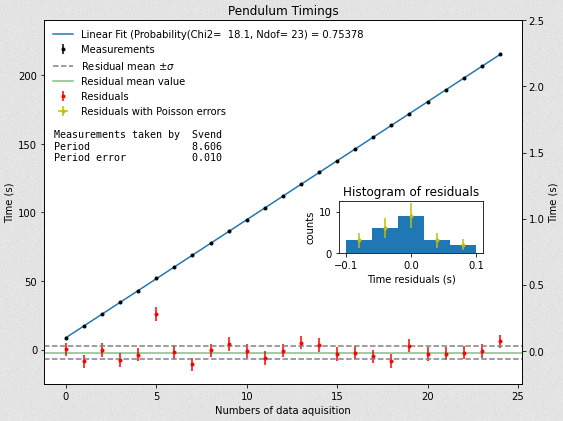
\includegraphics[width=\linewidth]{pendulum.jpeg}
\caption{A plot of the time data from the pendulum experiment. Also shown is a linear fit, alongside a histogram plot of the residual distribution. \label{fig:pendulumfit}}
\end{figure}

The first value obtained for $L$ was using the measuring tape, 
$L_{tape}=L_{top}-\frac{L_{m}}{2}$, where $L_{top}$ is the measure from the ceiling to the bottom of the mass, and $L_{m}$ is the height of the mass. A set of individual measures for this values are combined in a weighted mean, and the error $\sigma$ is obtained via propagation of the uncertainties. $L_{laser}$ was obtaining combining two measurements of $L_{top ,laser}$ measure from the hook to the floor, one measure of $L_{bottom ,laser}$, distance from the floor to the bottom of the mass, and $L_{m}$. Thus obtaining: $L_{tape}=(18.47 \pm 0.01)$ m, and $L_{mass}=(18.48 \pm 0.2)$ m. Which are combining with weighted mean to obtain the final value  $L_{tot}=(18.428 \pm 0.002)$ m. 
The fitting of the periods $T$ resulted in four different values with different uncertainties. In this case the individual error of the member is influenced by a series of factors, such as the clicking response time and eye coordination to determine if the mass passes our reference on the swing. Not knowing the uncertainties on the times these are obtained extrapolating the RMSE from a Gaussian fit of the residuals (corresponding to a difference between the data points and the fitted slope), that would determine the error, after dividing by the square root of the number of measurements. This four values are then combined in a weighted mean to obtain: $T=(8.605\pm 0.011)$ s. 
In the end $g$ can be calculated using those measures and the error propagation is: 

\begin{equation}
    \sigma_{g-pendulum}=\sqrt{\frac{64L^2\pi^4}{T^6}\sigma_T^2+\frac{16\pi^4}{T^4}\sigma_L^2}
\end{equation}
the value obtained is: $g=(9.82 \pm 0.03)\frac{m}{s^2}$
For each set of time measurements, after a linear fit of those, a $\chi^2$ and a probability, alongside the parameters of the fit are evaluated through \texttt{iminuit}\cite{iminuit}; exemplary values are shown in figure 2.
As described above an evaluation of the residual has been made ( inserts in Figure 2), in order to get the individual accuracy and the error associated with the data, via \texttt{iminuit} once again.
The final evaluation of g and its error has been done using \texttt{sympy}.

\begin{table}[H]
\centering
    \begin{tabular}{||c c c c||}
        \hline
        Variable & Value & Error & Impact on Error \\ 
        \hline\hline
        Length L  & 18.428 m & 0.002 m  & 6.4$\cdot10^{-7}$ $\frac{m^2}{s^4}$ \\ 
        \hline
        Time T  & 8.61 s & 0.02 s & 0.001 $\frac{m^2}{s^4}$ \\
        \hline
        \pmb{g} & 9.82 $\frac{m}{s^2}$ & 0.03 $\frac{m}{s^2}$ &   \\
        \hline
    \end{tabular}
    \caption{Variables and results from the pendulum experiment}
    \label{tab:pendulum}
\end{table}


\subsection{Ball on an incline}

\begin{figure}
\centering
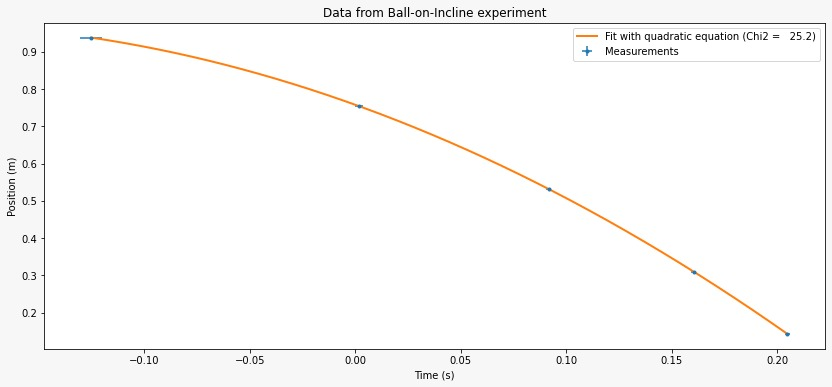
\includegraphics[width=\linewidth]{ball.jpeg}
\caption{A plot of the ball on incline data, alongside a $\chi ^2$ fit to a quadratic. \label{fig:fit_a}}
\end{figure}

% Topics to describe
% - (done) Describe the different setups we used and how many measurements each had (i.e. 3 for each direction x2 for different heights and +2 for vertical (1 measurement discarded, because it had only 4 peaks)
% - (done) Uncertainties on rail distances are unreasonably small -> rail distance uncertainties multiplied by a factor three to make it more reasonable
% - (done) How the passing times were determined
% - (done) How the quadratic fit was done
% - Make a good figure for the quadratic fit
% - (done) Why delta theta does not need to be calculated separately for us (should be in the theory part maybe?)
% - (done) Error propagation -> discussion
% - Systematic errors?
% - (done) Calculate g for the 5 different setups (show results in table)
% - Show that the found results are incoherent and are completely unreliable -> discussion

The acceleration of the ball was measured at five different angles: A set of measurements at the greatest inclination, a set at the same height but with the setup turned around, two sets at a smaller inclination taken in the same way as before, and a free fall set (i.e. $\theta = 90 \circ$).
Each set had three timing measurements. For the vertical fall one measurement was discarded because the ball did not trigger the last gate.

To find the passing times of the ball form the photo gate data, the \texttt{find\_peaks()} function from \texttt{SciPy} was used. That found the maximums of the voltage peaks.
The center and uncertainty of the peaks were then determined by finding the full width half maximum of each peak. The center was used as the passing time and the width as the uncertainty.

The passing times and gate positions were then used to perform a fit to the quadratic equation using \texttt{iminuit}.
Initially $\chi ^2$ values close to 30 were found. Only 5 data points were used per fit.
This indicated that the uncertainties on the gate positions were likely too low estimates.
Upon further consideration of the setup and how the positions were measured it was concluded that the uncertainties should be multiplied by at least a factor 3.
An example fit with $\chi ^2$ values is shown in figure \ref{fig:fit_a}.

The measurements of the $D_{ball}$, $d_{rail}$ and $\theta$'s can be found in tables \ref{tab:ball}, \ref{tab:rail}, \ref{tab:angles1} and \ref{tab:angles2} respectively.

Using weighted averages where possible gives the values of $g$ shown in table \ref{tab:g_incline}.
The equation for the error propagation for $g$ of the ball on incline is given by
% I'm afraid this is the old version
%\begin{equation}
%    \begin{split}
%        \sigma_{g-incline}^2=[1+\frac{2}{5}\frac{D_{ball}^2}{D_{ball}^2-D_{rail}^2}]\frac{1}{\sin{(\theta+\Delta\theta)}^2}\sigma_a^2\\
%        +a^2[1+\frac{2}{5}\frac{D_{ball}^2}{D_{ball}^2-D_{rail}^2}]\frac{\cos{(\theta+\Delta\theta)}^2}{\sin{(\theta+\Delta\theta)}^4}\sigma_{\theta}^2\\
%        +a^2[1+\frac{2}{5}\frac{D_{ball}^2}{D_{ball}^2-D_{rail}^2}]\frac{\cos{(\theta+\Delta\theta)}^2}{\sin{(\theta+\Delta\theta)}^4}\sigma_{\Delta\theta}^2\\
%        +\frac{a^2}{\sin{(\theta+\Delta\theta)}^2}(\frac{4}{5}\frac{D_{ball}}{D_{ball}^2-D_{rail}^2}-\frac{4}{5}\frac{D_{ball}^3}{D_{ball}^2-D_{rail}^2})^2\sigma_{D_{ball}}^2\\
%        +\frac{16a^2D_{ball}^4D_{rail}^2}{25\sin{(\theta+\Delta\theta)}^2({D_{ball}^2-D_{rail}^2})^4}\sigma_{rail}^2
%    \end{split}
%\end{equation}

% New version time
\begin{equation}
    \begin{split}
        \sigma_{g-incline}^2 = \left(1 + \frac{2}{5}\frac{D_{ball}^2}{D_{ball}^2 - d_{rail}^2} \right)^2 \frac{1}{\sin{(\theta)}^2}\sigma_a^2 \\
        + a^2 \left(1 + \frac{2}{5}\frac{D_{ball}^2}{D_{ball}^2-d_{rail}^2}\right)^2 \frac{\cos{(\theta)}^2}{\sin{(\theta)}^4} \sigma_{\theta}^2\\
        + \frac{16 a^2}{25 \sin{(\theta)}^2} \left( \frac{D_{ball}}{D_{ball}^2-d_{rail}^2} - \frac{D_{ball}^3}{( D_{ball}^2 - d_{rail}^2 )^2} \right)^2 \sigma_{D_{ball}}^2\\
        + \frac{16 a^2 D_{ball}^4 d_{rail}^2}{25\sin{(\theta)}^2 \left({D_{ball}^2 - d_{rail}^2}\right)^4} \sigma_{d_{rail}}^2
    \end{split}
\end{equation}

\begin{table}[H]
\centering
    \begin{tabular}{||c c c||}
        \hline
         Method & Value & Error \\ 
        \hline\hline
        Angle $15.7 ^\circ$ & 8.67 $\frac{m}{s^2}$ & 0.07 $\frac{m}{s^2}$\\
        \hline
        Angle $15.0 ^\circ$ & 8.75 $\frac{m}{s^2}$ & 0.08 $\frac{m}{s^2}$\\
        \hline
        Angle $5.4 ^\circ$ & 8.30 $\frac{m}{s^2}$ & 0.16 $\frac{m}{s^2}$\\
        \hline
        Angle $5.5 ^\circ$ & 7.40 $\frac{m}{s^2}$ & 0.14 $\frac{m}{s^2}$\\
        \hline
        Vertical & 9.49 $\frac{m}{s^2}$ & 0.05 $\frac{m}{s^2}$\\
        \hline
    \end{tabular}
    \caption{Different measurements of g from ball on incline}
    \label{tab:g_incline}
\end{table}



\section{Discussion}

%The two values of $g$ obtained in this experiment are:  $g_{pendulum}=(9.82 \pm 0.04)\frac{m}{s^2}$ and $g_{ball on incline}=(9.486 \pm 0.017)\frac{m}{s^2}$, which are respectively $0.11  \sigma_{g,pendulum}$ and $19.4  \sigma_{g,incline}$ away from the value of reference for $g$ in Copenhagen, which is $g_{ref}= 9.81 54960 \pm 0.0000002 \frac{m}{s^2} $\cite{DTU}. 

The value of $g$ obtained in the pendulum experiment is:  $g_{pendulum}=(9.82 \pm 0.03)\frac{m}{s^2}$, which is $0.11  \sigma_{g,pendulum}$ away from the value of reference in Copenhagen; $g_{ref}= 9.81 54960 \pm 0.0000002 \frac{m}{s^2} $\cite{DTU}.
The errors on the pendulum measurements can be seen in table \ref{tab:pendulum}, where it's clear that the dominant factor in the propagated error for $g$ is given by the error on $T$, and thus for obtaining the most precise possible value for $g$ one should focus on reducing the error on the timing of the period as much as possible.

For the ball on incline the error discussion is a bit more delicate.
From table \ref{tab:g_incline} it is immediately clear that there is a disagreement between the different configurations of the experiment.
The calculated uncertainties are too small to cover this disagreement.

It is immediately clear from the formula for error propagation that there are many more factors that play a role here.
From the last column in table \ref{tab:incline15degr} it becomes clear that the ball diameter is the only parameter that does not play a major role in the uncertainty on $g$.
 
\begin{table}[H]
\centering
\begin{tabular}{||c c c c||} 
 \hline
 Variable & Value & Error & Impact on Error \\  
 \hline\hline
 Angle $\theta$ & 15.5 $^\circ$ & 0.1 $^\circ$ & 1.72 $\cdot 10^{-2}$ $\frac{m^2}{s^4}$ \\ 
  \hline
 Rail Diameter & 0.61 $\cdot 10^{-3}$  m & 0.01 $\cdot 10^{-3}$ m & 1.79 $\cdot 10^{-2}$ $\frac{m^2}{s^4}$ \\
  \hline
 Ball Diameter & 1.27 $\cdot 10^{-3}$ m & 0.01 $\cdot 10^{-3}$ m & 0.10 $\cdot 10^{-2}$ $\frac{m^2}{s^4}$ \\
  \hline
 Acceleration a & 1.54 $\frac{m}{s^2}$  & 0.01 $\frac{m}{s^2}$ & 2.00 $\cdot 10^{-2}$ $\frac{m^2}{s^4}$ \\
 \hline
 \pmb{g} & 8.74 $\frac{m}{s^2}$  & 0.08 $\frac{m}{s^2}$ & \\
 \hline
\end{tabular}
\caption{Variables and results from one of the ball on incline experiments}
\label{tab:incline15degr}
\end{table}

The discrepancy between the different values for $g$ can not simply be explained by the uncertainties on our measurements.
It is likely that there were systematic uncertainties in our setup causing the problems.
One example could be the drag of the ball while it rolled down the incline. 
However, that can not be the only factor, since the vertical case does not suffer from this drag, but it is still not close enough to the commonly accepted value for $g$.



Given these experimental setups it's more convenient to measure $g$ using the pendulum, where there are less factors in play and it's easier to reduce the error by focusing on a single factor, instead of optimising the precision on many elements like happens in the ball on incline.
For the contribution on the error was taken into consideration the measure: $\sigma_{g}^2=(A)\sigma_{T}^2+(B)\sigma_L^2$, and $A)\sigma_{T}^2$ and $(B)\sigma_L^2$ are defined as the contribution to the error of $T$ and $L$ respectively.







\section{Conclusion}
After measuring the gravitational acceleration constant in two different ways the results obtained are: $g_{pendulum}=(9.82 \pm 0.03)\frac{m}{s^2}$ and the best result for the ball on incline $g_{ball on incline}=(9.47 \pm 0.05)\frac{m}{s^2}$. That compared to the known value tells us that the pendulum experiment was more successful, being more accurate in getting the central value for $g$ and a smaller error. Since the closest value obtained for $g_{ball on incline}$ is $19.4 \sigma_{g,incline}$ of distance from the reference value, all measurements from the ball on incline should be disregarded. This is probably due to a systematic error, not spotted because of how there isn't one parameter in the equation dominating the other terms, and how many factors were into play when conducting the experiment.




\section{Appendix}


\begin{table}[H]
\centering
\begin{tabular}[t]{lcc}
\hline
&Value &Error\\
\hline
1&8.607s&0.002s\\
2&8.614s&0.002s\\
3&8.601s&0.009s\\
4&8.602s&0.002s\\
\hline
\end{tabular}
\caption{Period T}
\label{tab:periods}
\end{table}

\begin{table}[H]
\centering
\begin{tabular}[t]{lcc}
\hline
&Value &Error\\
\hline
1&18.48m&0.02m\\
2&18.496m&0.0015m\\
3&18.492m&0.001m\\
4&18.492m&0.001m\\
\hline
\end{tabular}
\caption{Distance from Hook to Bottom of the Mass - Tape}
\end{table}

\begin{table}[H]
\centering
\begin{tabular}[t]{lcc}
\hline
&Value &Error\\
\hline
1&0.03000m&5.e-05m\\
2&0.03005m&5.e-05m\\
3&0.0301m&1.e-04m\\
4&0.0299m&5.e-05m\\
\hline
\end{tabular}
\caption{Height of the Mass}
\end{table}

\begin{table}[H]
\centering
\begin{tabular}[t]{lcc}
\hline
&Value &Error\\
\hline
1&18.766m&0.001m\\
2&18.762m&0.0005m\\
\hline
\end{tabular}
\caption{Distance Hook to Floor - Laser}
\end{table}

\begin{table}[H]
\centering
\begin{tabular}[t]{lcc}
\hline
&Value &Error\\
\hline
1&0.320m&0.001m\\
\hline
\end{tabular}
\caption{Distance Floor to Mass - Laser}
\end{table}

\begin{table}[H]
    \centering
    \begin{tabular}{lcc}
    \hline
    &Value &Error\\
    \hline
     1 & 1.27 mm & 0.01 mm \\
     2 & 1.27 mm &  0.01 mm\\
    \hline
    \end{tabular}
    \caption{Ball Diameter}
    \label{tab:ball}
\end{table}

\begin{table}[H]
    \centering
    \begin{tabular}{lcc}
    \hline
    &Value &Error\\
    \hline
     1 & 0.62 mm & 0.02 mm \\
     2 & 0.62 mm & 0.01 mm \\
    \hline
    \end{tabular}
    \caption{Rail Diameter}
    \label{tab:rail}
\end{table}

\begin{table}[H]
    \centering
    \begin{tabular}{lcc}
    \hline
    &Value &Error\\
    \hline
    \hline
    Length 1&&\\
    \hline
     1 & 278.5 mm & 0.5 mm \\
     2 & 278.0 mm & 0.1 mm \\
     3 & 278.5 mm & 0.5 mm \\
    \hline
    \hline
    Length 2&&\\
    \hline
    1 & 31 mm & 1 mm \\
    2 & 31 mm & 1 mm \\
    \hline
    \hline
    Height &&\\
    \hline
    1 & 926 mm & 1 mm \\
    2 & 927 mm & 0.5 mm \\
    3 & 926 mm & 1 mm \\
    \hline
    \end{tabular}
    \caption{Lengths in triangle}
    \label{tab:my_label}
\end{table}

\begin{table}[H]
    \centering
    \begin{tabular}{lcc|cc}
    \hline
    & Gio. Normal && Gio. Flipped &\\
    \hline
    &Value &Error & Value & Error\\
    \hline
    \hline
    Setup Normal &&&&\\
    \hline
    1 & 105.5$^{\circ}$ & 0.2$^{\circ}$ & 105.9$^{\circ}$ & 0.2$^{\circ}$\\
    2 & 105.5$^{\circ}$ & 0.2$^{\circ}$ & 105.1$^{\circ}$ & 0.25$^{\circ}$\\
    3 & 105.6$^{\circ}$ & 0.1$^{\circ}$ & 105.8$^{\circ}$ & 0.1$^{\circ}$\\
    4 & 105.4$^{\circ}$ & 0.2$^{\circ}$ & 105.9$^{\circ}$ & 0.2$^{\circ}$\\
    \hline
    \hline
    Setup Flipped &&&&\\
    \hline
    1 & 104.9$^{\circ}$ & 0.1$^{\circ}$ & 105.5$^{\circ}$ & 0.1$^{\circ}$\\
    2 & 105.9$^{\circ}$ & 0.25$^{\circ}$ & 105.0$^{\circ}$ & 0.05$^{\circ}$\\
    3 & 105.8$^{\circ}$ & 0.1$^{\circ}$ & 105.05$^{\circ}$ & 0.25$^{\circ}$\\
    4 & 105.7$^{\circ}$ & 0.2$^{\circ}$ & 105.1$^{\circ}$ & 0.1$^{\circ}$\\
    \hline
    \end{tabular}
    \caption{Gionometer Measurements. All angles should be subtracted by 90$^{\circ}$ to find the angle of the rail due to the way the goniometer was read.}
    \label{tab:angles1}
\end{table}

\begin{table}[H]
    \centering
    \begin{tabular}{lcc}
    \hline
    &Value &Error\\
    \hline
    \hline
    Start 1&&\\
    \hline
     1 & 98.4 cm & 0.1 cm \\
     2 & 98.5 cm & 0.05 cm \\
     3 & 98.44 cm & 0.05 cm \\
     4 & 98.4 cm & 0.1 cm\\
    \hline
    \hline
    Gate 1&&\\
    \hline
     1 & 98.3 cm & 0.1 cm \\
     2 & 93.35 cm & 0.05 cm \\
     3 & 93.32 cm & 0.05 cm \\
     4 & 93.3 cm & 0.1 cm\\
     \hline
     \hline
     Gate 2&&\\
     \hline
     1 & 75.4 cm & 0.1 cm \\
     2 & 75.44 cm & 0.05 cm \\
     3 & 75.44 cm & 0.05 cm \\
     4 & 75.4 cm & 0.1 cm\\
     \hline
     \hline
     Gate 3&&\\
     \hline
     1 & 53.3 cm & 0.1 cm \\
     2 & 53.3 cm & 0.05 cm \\
     3 & 53.25 cm & 0.05 cm \\
     4 & 53.3 cm & 0.1 cm\\
     \hline
     \hline
     Gate 4&&\\
     \hline
     1 & 30.9 cm & 0.1 cm \\
     2 & 30.9 cm & 0.05 cm \\
     3 & 30.95 cm & 0.05 cm \\
     4 & 30.9 cm & 0.1 cm\\
     \hline
     \hline
     Gate 5&&\\
     \hline
     1 & 14.2 cm & 0.1 cm \\
     2 & 14.15 cm & 0.05 cm \\
     3 & 14.7 cm & 0.05 cm \\
     4 & 14.1 cm & 0.1 cm\\
     \hline
    \end{tabular}
    \caption{Gate positions}
    \label{tab:my_label}
\end{table}

\begin{table}[H]
    \centering
    \begin{tabular}{lcc|cc}
    \hline
    & Gio. Normal && Gio. Flipped &\\
    \hline
    &Value &Error & Value & Error\\
    \hline
    \hline
    Setup Normal &&&&\\
    \hline
    1 & 95.6$^{\circ}$& 0.1$^{\circ}$ & 95.2$^{\circ}$& 0.1$^{\circ}$\\
    \hline\hline
    Setup Flipped &&&&\\
    \hline
    1& 95$^{\circ}$ & 0.1$^{\circ}$ & 96 $^{\circ}$ & 0.1$^{\circ}$\\
    \hline
    \end{tabular}
    \caption{Gionometer Measurements for the second incline experiment. All angles should be subtracted by 90$^{\circ}$ to find the angle of the rail due to the way the goniometer was read.}
    \label{tab:angles2}
\end{table}


\begin{thebibliography}{99}  
\bibitem{setup}
Labguide homepage, URL: \url{https://www.nbi.dk/~petersen/Teaching/Stat2021/Project/project.html}
\bibitem{iminuit}
iminuit, URL: \url{https://iminuit.readthedocs.io/en/latest/about.html}
\bibitem{GitHub}
GitHub Depository, URL: \url{https://github.com/vjbAvanzi/Group12_AppStat2021}
{https://iminuit.readthedocs.io/en/latest/about.html}
\bibitem{DTU}
DTU NSI measure for g, URL: \url{http://outer.space.dtu.dk/gravity/DK_0101_GI101_CopenhagenGamlehave.pdf}

\bibitem{Barlow}
RJ Barlow, A Guide to the Use of Statistical Methods in the Physical Sciences


\end{thebibliography}

\end{document}                                                
